\section{Methods}
\label{sec:methods}

All events in a team sport are performed in the same scene by the same set
of players. The only basis for differentiating these events is the action
pefromed by a small subset of people at a given time.  For instance, a
``steal" event in basketball is completely defined by the action of the player attempting to
pass the ball and the player stealing from him.  To understand such an event,
it is sufficient to observe only these players pariticipating in the event.

This motivates us to build a model which can reason about an event by focusing
on specific people during the different phases of the event.
In this section, we describe our unified model for classifying events
and simultaneously identifying the key players.

<<<<<<< HEAD
\begin{figure}[t!]
\begin{center}
    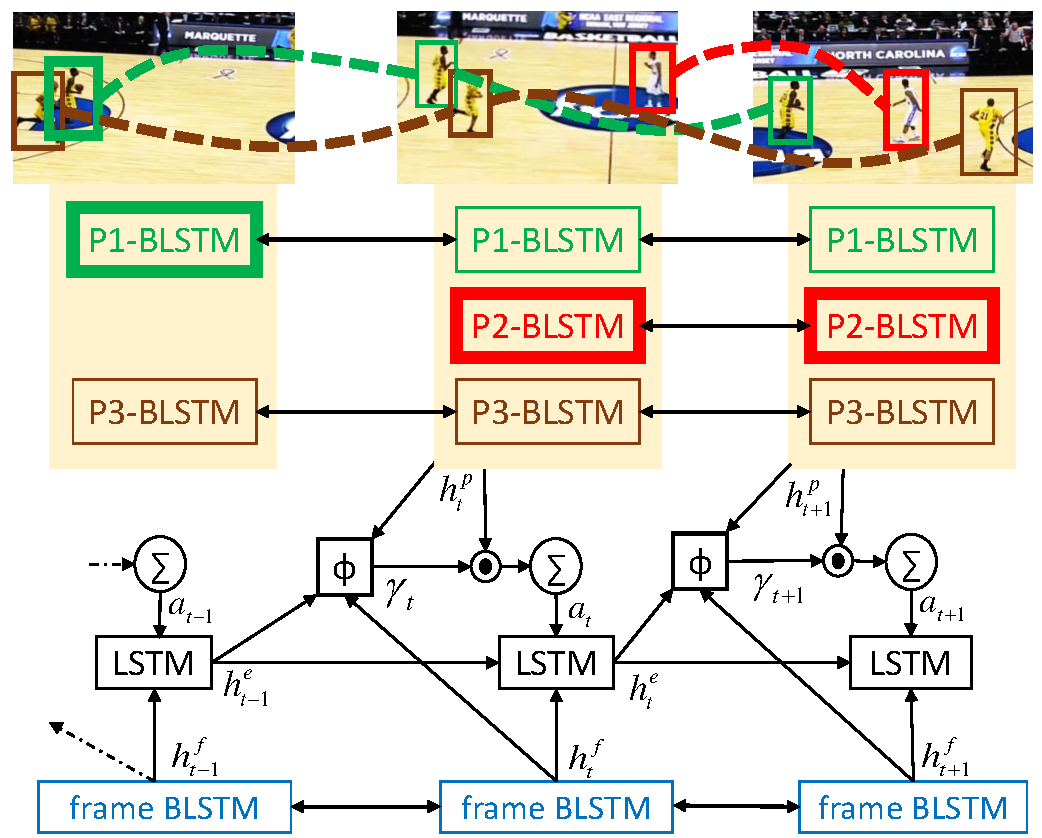
\includegraphics[width=3 in]{images/system_figure_1_cropped_v2.pdf}
\end{center}
   \caption{Our attention model where each player track is represented by the
     corresponding BLSTM. The variables in the model are explained in the
     methods section.  BLSTM stands for ``bidirection long short term memory''.
}
\label{fig:model}
\end{figure}
=======
We used AMT to annotate the location of all the players in a subset \KEVIN{HOW BIG?}
of the training data. We then trained a Multibox detector to detect players,
and ran this on all the training and test videos.  We kept all detections above
a confidence of 0.5 per frame; this resulted in between 0 and 10 (\KEVIN{10?}) bounding
boxes per frame. 
%These detected player bounding boxes will also by the
%multi-box model will be made available in the dataset.

\eat{
Given a set of basketball video clips, we first preprocess the clips to extract
player bounding boxes and features. We train a Multibox model \cite{} to detect
basketball players with bounding-box annotations collected on a subset of
training video frames. This model is then run on all frames of the training and
test videos to extract player bounding boxes.
>>>>>>> 9217d0e650c738bf0d9a80541fa1521fcbd746a5


\subsection{Feature extraction}

<<<<<<< HEAD
Each video-frame is represented by a feature vector $f_t$, which is the activation
of the last fully connected layer of Inception7 network
\cite{Ioffe_arxiv15,Inception7}.  In addition, we compute spatially localized features
for each person in the frame. In particular,
$p_{ti}$ contains both appearance and spatial information for the $i$'th
player bounding box in frame $t$. Similar to the RCNN object detector\cite{},
=======
Frame $t$ is represented by a feature vector $f_t$, which is the activation
of the last fully connected layer of GoogLeNet \cite{} trained on ImageNet
\cite{}.  In addition, we compute spatially localized features.  In particular,
$p_{ti}$ contains both appearance and spatial information for the $i$'th
player's bounding box in frame $t$. Similar to the RCNN object detector\cite{},
>>>>>>> 9217d0e650c738bf0d9a80541fa1521fcbd746a5
the appearance features were extracted by feeding
the cropped and resized player region from the frame through the Inception7 network and
spatially pooling the response from a lower layer. The spatial feature
<<<<<<< HEAD
corresponds to a spatial histogram indicating the bounding box location.
=======
corresponds to a 32 x 32 spatial histogram, combined with a spatial
pyramid,
to indicate the bounding box location at multiple scales.

>>>>>>> 9217d0e650c738bf0d9a80541fa1521fcbd746a5

\subsection{Event classification}

Given $f_t$ and $p_{ti}$ for $t=1:T$, our goal
is to train the model to classify the clip into one of 11 categories. As a side
effect of the way we construct our model, we will also be able to identify the
key players in each frame.

First we compute a global context feature for each frame, $h_t^f$, derived from
a bidirectional LSTM applied to the frame-level feature as shown in Fig.~\ref{fig:model}.
This is a concatenation of the hidden states from the forward and reverse LSTM
components of a BLSTM and can be compactly represented as:
\[
  h_t^f = \mbox{BLSTM}_{frame}(h_{t-1}^f, h_{t+1}^f, f_t).
\]Please refer to Graves et al. \cite{Graves_2013} or the supp. material
for the full equations.

Next we use use a unidirectional LSTM to represent the state of the
event at time $t$:
\[
h_t^e = \mbox{LSTM}(h_{t-1}^e, h_t^f, a_t)
\]
where $a_t$ is a feature vector derived from the players, as we
describe below.
From this, we can predict the class label for the clip using
$w_k^{\transpose} h_t^e$,
where the weight vector corresponding to
class $k$ is denoted by $w_k$.
 We measure the loss as follows:
\begin{equation}
  L =   \frac{1}{2} \sum_{t=1}^T \sum_{k = 1}^K \max (0, 1 - y_k w_k^{\transpose} h^e_t)^2
\end{equation} 
where $y_k$ is $1$ if the video belongs to class $k$,
else it is $-1$.

\subsection{Attention models}
<<<<<<< HEAD
\VIGNESH{I have added back my original motivation section for the attention model. I felt
that the section was otherwise very descriptive and didn't motivate the method
sufficiently}

Unlike past attention models \cite{}, we need to attend to a different set of
=======
Unlike past attention models, we need to attend to a different set of
>>>>>>> 9217d0e650c738bf0d9a80541fa1521fcbd746a5
features at each time-step. There are two key issues to address in this
setting.

First, although we have different detections in each frame, they
can be connected across the frames through an object tracking
method. This could potentially lead to better feature representation of the
players.

Second, player attention depends on the state of the event and needs to evolve
with the event.  For instance, during the start of a ``free-throw" it is
important to attend to the player making the shot. However, towards the end of
the event the success or failure of the shot can be judged by observing the
person in possession of the ball.

<<<<<<< HEAD
With these issues in mind, we first present our model which uses player tracks
and learns a BLSTM based representation for each player track. Next, we also
present a simple tracking-free baseline model.

\noindent \textbf{Attention model with tracking}

We first associate the detecitons
belonging to the same player into tracks using a standard
tracking method. We use a KLT tracker combined with
bipartite graph matching \cite{} to perform the data association.

We use a separate BLSTM to learn a better context based
representation for each player at a given time-step.
The latent representation of player $i$ in frame $t$ is
given by the hidden state
$h_{ti}^p$ of the BLSTM across the player-track:
\[
  h_{ti}^p = \mbox{BLSTM}_{track}(h_{t-1,i}^p, h_{t+1,i}^p, p_{ti}).
\]

To compute $a_t$, we take a convex combination of the player features:
=======
With these issues in mind, we explore two models:
one without a person  tracker and the other using a person tracker.


\noindent \textbf{Attention model without tracking}
Here, we treat the detections in each frame as independent from other
frames.  This alows the model to be more flexible in switching attention
between players as the event progresses.  As we later observe empirically, this
leads to better interpretability.  Also, the model does not suffer from
tracking errors.

To compute $a_t$, we take a convex combination of the player features:
\begin{eqnarray} 
\label{eq:notrack}
  a_t^{notrack} & = & \sum_{i=1}^{N_t} \gamma_{ti}^{notrack} p_{ti} 
\\ \nonumber
  \gamma_{ti}^{notrack} & = & \text{softmax} \left(\phi\left(h^f_t, p_{ti}, h^e_{t-1}\right); \tau\right),
\end{eqnarray}
where $N_t$ is the number of detections in frame $t$,
and $\phi()$ is a 
multi layer perceptron $\phi$, 
and $\tau$ is the softmax temperature parameter,
similar to
\cite{Bahdnau_arxiv14}. 
This model is illustrated in Figure~\ref{fig:model}(a).

\begin{figure*}[t!]
\begin{center}

   \subfigure[Attention without tracks]{
                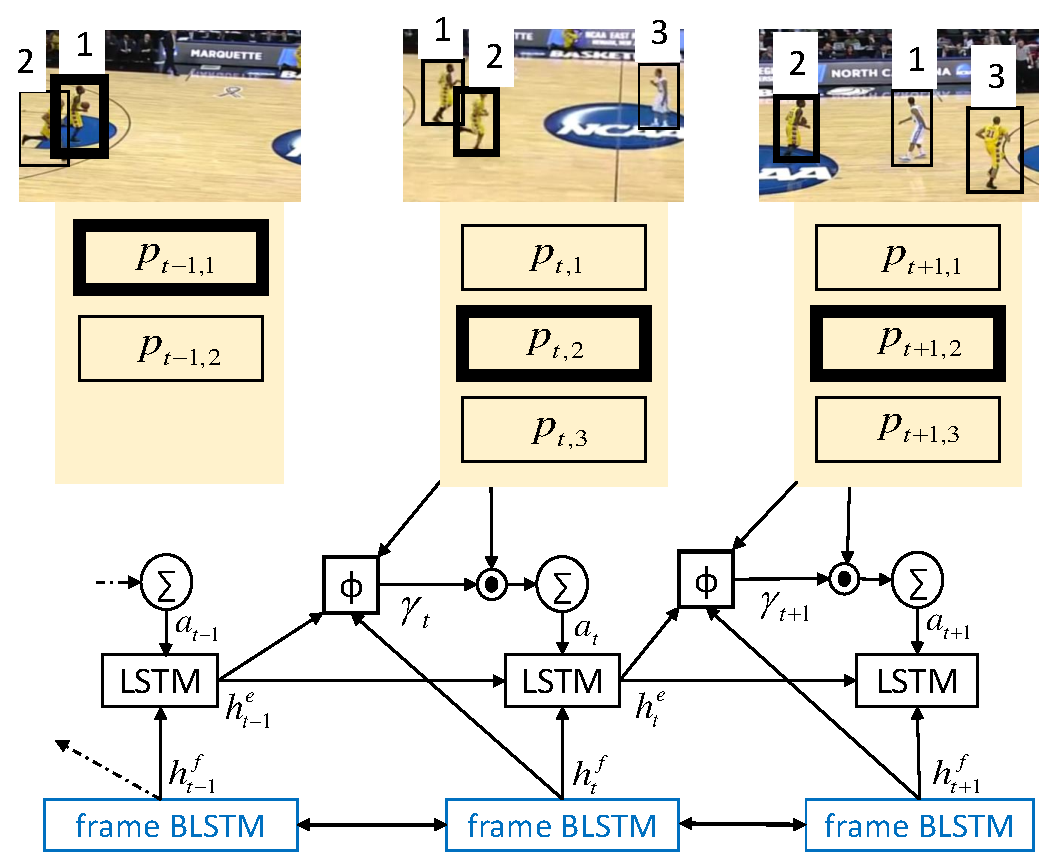
\includegraphics[width=3 in]{images/system_figure_2_cropped_v2.pdf}
                \label{fig:heatmap_ft}
    }
   \subfigure[Attention with tracks]{
                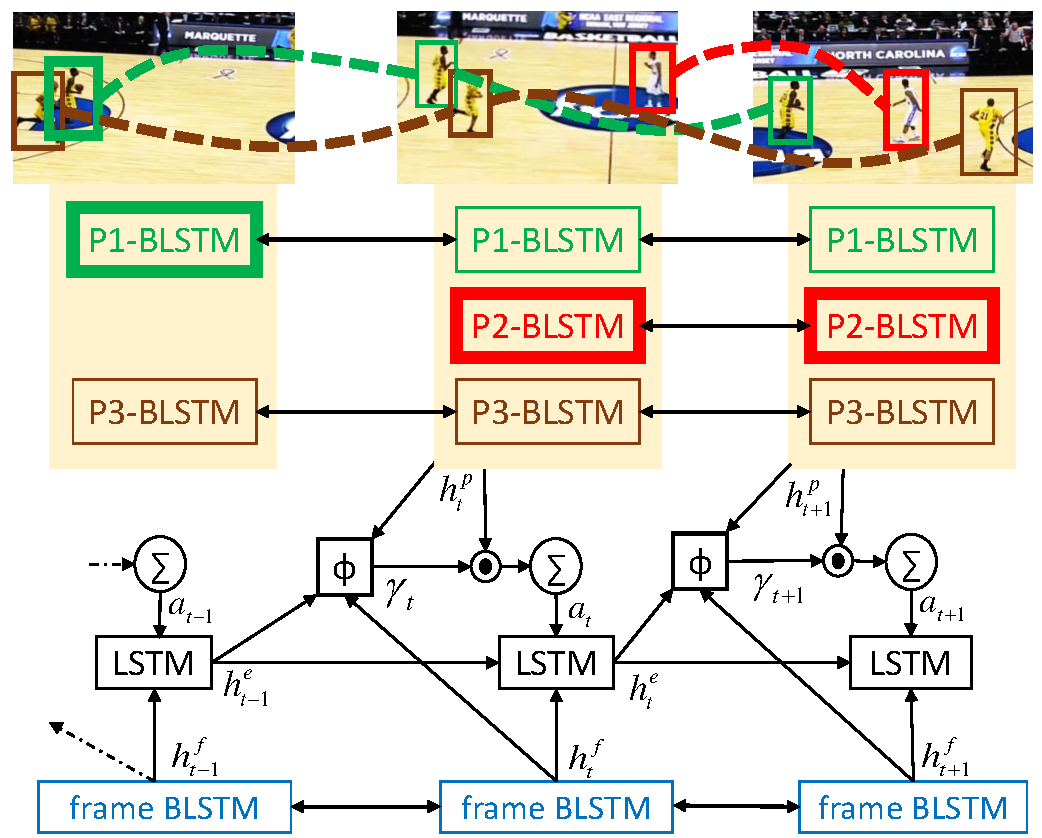
\includegraphics[width=3 in]{images/system_figure_1_cropped_v2.pdf}
                \label{fig:heatmap_lp}
    }
\end{center}
   \caption{Our attention models (a) without tracks and (b) with tracks.
BLSTM stands for ``bidirectional long short term memory''.
See text for details.
}
\label{fig:model}
\end{figure*}


\noindent \textbf{Attention model with tracking}
One potential weakness of the previous model is that the
player being attended to can change from frame to frame.
An alternative approach is to first associated detections
belonging to the same player into tracks using a standard
tracking method. We use a standard KLT tracker combined with
bipartite graph matching to perform the data association
\cite{Veenman_PAMI2001}.
We then compute the attention scores as shown below:
%
>>>>>>> 9217d0e650c738bf0d9a80541fa1521fcbd746a5
\begin{eqnarray} 
\label{eq:track}
  a_t^{track} & = & \sum_{i=1}^{N_t} \gamma_{ti}^{track} p_{ti} 
\\ \nonumber
  \gamma_{ti}^{track} & = & \text{softmax} \left(\phi\left(h^f_t, h^p_{ti}, h^e_{t-1}\right); \tau\right),
<<<<<<< HEAD
\end{eqnarray}where $N_t$ is the number of detections in frame $t$, and $\phi()$ is a 
multi layer perceptron, similar to \cite{Bahdnau_arxiv14}. $\tau$ is the softmax temperature parameter.
=======
\end{eqnarray}
This is the same as before, except 
that instead of the observed player features $p_{ti}$, 
we use $h_{ti}^p$, which is the latent representation of player $i$ in frame
$t$ computed using a BLSTM across tracks:
\[
  h_{ti}^p = \mbox{BLSTM}(h_{t-1,i}^p, h_{t+1,i}^p, p_{ti})
\]
This model is illustrated in Figure~\ref{fig:model}(b).
Below  we show that although this method gives slightly better
performance at event classification, it gives worse results for player
identification, because it is sensitive to tracking errors, and
is often unable to switch between players within an event.



\eat{
\subsection{Attention models}

Unlike past attention models \cite{}, we need to attend to a different set of
features at each time-step. There are two key issues to address in this
setting.

First, although we have different set of detections in each frame, the player
detections can be connected across the frames through an object tracking
method. This could potentially lead to better feature representation of the
players.

Second, player attention depends on the state of the event and needs to evolve
with the event.  For instance, during the start of a ``free-throw" it is
important to attend to the player making the shot. However, towards the end of
the event the success or failure of the shot can be judged by observing the
person in posession of the ball.
>>>>>>> 9217d0e650c738bf0d9a80541fa1521fcbd746a5

This model is illustrated in Figure~\ref{fig:model}.
Later, we show that this method achieves better
performance at event classification and detection compared to a
tracking-free model. However, it could result in slightly worse ``key player"
identifcation due to tracking errors.

\noindent \textbf{Attention model without tracking}
Here, we treat the detections in each frame to be independent from other
frames.  This alows the model to be more flexible in switching attention
between players as the event progresses.  As we later observe empirically, this
leads to better interpretability.  Also, the model does not suffer from
tracking errors.

We then compute the attention based player feature as shown below:
\begin{eqnarray} 
\label{eq:notrack}
  a_t^{notrack} & = & \sum_{i=1}^{N_t} \gamma_{ti}^{notrack} p_{ti} 
\\ \nonumber
  \gamma_{ti}^{notrack} & = & \text{softmax} \left(\phi\left(h^f_t, p_{ti}, h^e_{t-1}\right); \tau\right),
\end{eqnarray}
<<<<<<< HEAD
=======

While this provides a more consistent representation for the players across frames,
this model could suffer from wrong associations due to trakcing. This in turn makes
the interpretation of attention scores more difficult.


\subsection{LSTM event classifier}
Given a video $v$, we pass the frame-level features $f_t$ at time $t$ through a
Bidirectional Long Short-Term Memory (BLSTM) network. This helps in combining
contextual information from adjacent frames to provide a better frame
representation.  Let the hidden state of this BLSTM at time $t$ be denoted by
$h^f_t$.  This is the concatenated hidden state from both the forward and the
reverse LSTMS of the BLSTM. Refer to supp.  material for more details.

In order to attend to specific players in each frame, we pass the player features
through our attention model to generate an attention weighted player feature
$a_t$. The attention model is the main contribution of our work
and is explained in detail in the next section.

We feed the concatenated vector $[h^f_t, a_t]$ to a final event classification
LSTM, similar to the LRCN \cite{} model for video classification. Let
the hidden state of this LSTM at time $t$ be represented by $h^e_t$.  We then
train the model by minimizing the following one-vs-all hinge loss:

\begin{equation}
  L = \sum_{k = 1}^K \max (0, 1 - y_k w_k \cdot h^e_t)^2,
\end{equation} where $y_k$ is $1$ if the video belongs to class $k$,
else it is $-1$, and the weight vector corresponding to
class $k$ is denoted by $w_k$.
}

\subsection{Implementation details}

 We used a hidden state dimension of $256$ for all the LSTM and
BLSTM RNNs, an embedding layer with ReLU non-linearity and $256$ dimension for
embedding the player features and frame features before feeding to the RNNs.
We used $32 \times 32$ bins with spatial pyramid pooling for the player appearance
feature.
All the event videos clips were four seconds long and subsampled to 6fps.  The
$\tau$ value was set to $0.25$ for the attention softmax weighting. We used a
batch size of $128$, learning rate of $0.005$ which was reduced by a factor of
$0.1$ every $10000$ iterations with RMSProp\cite{RMSProp}. The models were trained on
a cluster of $20$ GPUs for $100k$ iterations over one day.
The hyperparameters were chosen by cross-validating on the
validation set.
>>>>>>> 9217d0e650c738bf0d9a80541fa1521fcbd746a5
